% !TXS template
\documentclass[german]{article}
\usepackage[T1]{fontenc}
\usepackage[utf8]{inputenc}
\usepackage{lmodern}
\usepackage[a4paper]{geometry}
\usepackage{babel}

\usepackage{amsmath}
\usepackage{amsfonts}
\usepackage{amssymb}
\usepackage{amsthm}

\usepackage{mathtools}

\title{Mathematische Logik 2:\\Vorlesungmitschrift}
\author{Theodor Teslia}
\date{}


\newtheoremstyle{break}
{\topsep}{\topsep}%
{}{}%
{\bfseries}{}%
{\newline}{}%

\theoremstyle{break}
\newtheorem{example}{Beispiel}[section]

\newtheoremstyle{def_style}
{\topsep}{\topsep}%
{}{}%
{\bfseries}{}%
{\newline}{}%

\theoremstyle{def_style}
\newtheorem{definition}{Definition}[section]

\theoremstyle{def_style}
\newtheorem{satz}{Satz}[section]

\newtheoremstyle{lemma_style}
{\topsep}{\topsep}%
{}{}%
{\itshape}{:}%
{ }{}%

\theoremstyle{lemma_style}
\newtheorem{lemma}{Lemma}[subsection]

\usepackage{tikz}

\newcommand{\Pot}[1]{\mathcal{P}(#1)}

\begin{document}

\maketitle

\tableofcontents

\section{Mengenlehre}

\glqq Aus dem Paradies, das Cantor uns geschaffen, soll uns niemand vertreiben können.\grqq{}\\
(David Hilbert, 1926) 

\subsection{Mengen und Klassen}

Reine Mengen sind Kollektion an Objekten, die ebenfalls wieder Mengen sind, als Alternative lassen sich Mengen ausgehend von Urelementen definieren.
\\
Wie führt die Mathematik Objekte ein?
\begin{itemize}
	\item Explizite Konstruktion aus schon vorhandenen Objekten, bspw. Konstruktion der rationalen, reellen und komplexen Zahlen, ausgehend von den ganzen und natürlichen.
	\item Axiomatisches formulieren von gewünschten Eigenschaften der Objekte und betrachte alle Objekte, die die Eigenschaften erfüllen, bspw. Gruppen, Vectorräume, ...
\end{itemize}

\begin{definition}[Mengen]
	Intuitiv sind Mengen \textit{Kollektionen von Objekten}, die selbst wieder Mengen sind. 
	
	$a\in b$: $a$ ist ein Element in der Menge $b$.
	
	$a \subseteq b$: Jedes Element von $a$ ist auch in $b$.
	\\
	Eine Konstruktive Definition von aller Menge könnte wie folgt aussehen:\\ $\{\emptyset\}, \{\emptyset,\{\emptyset\}\}, \{\{\emptyset\}\}$ \textit{usw.}
	Problem: Wie sieht dieses \textit{usw.} aus?
\end{definition}


Mengen lassen sich auch als Bäume darstellen. Dies lässt sich in Abbildung \ref{Mengenbaum} Beispielhaft für die Menge $\{\; \emptyset, \; \{\emptyset\}, \; \{\emptyset,\{\emptyset\}\}\;\}$ erkennen. 

\begin{figure}[h]
	\begin{center}
		\begin{tikzpicture}
			\node {$\bigcirc$}
			child {node {$\emptyset$}}
			child {node {$\bigcirc$}
				child {node {$\emptyset$}}}
			child {node {$\bigcirc$}
				child {node {$\emptyset$}}
				child {node {$\bigcirc$}
					child {node {$\emptyset$}}}};
		\end{tikzpicture}
	\end{center}
\caption{Darstellung der Menge $\{\; \emptyset, \; \{\emptyset\}, \; \{\emptyset,\{\emptyset\}\}\;\}$ als Baum}
\label{Mengenbaum}
\end{figure}

\begin{definition}[Hereditär endliche Mengen]
	Die \textit{hereditär endlichen Mengen} ($HF$) bilden eine Miniaturversion der Mengenlehre. Es gilt $HF_0\subset HF_1 \subset HF_2 \subset \dots$. Definiert sind diese Mengen induktiv als $HF_0\coloneqq \emptyset$ und $HF{n+1}\coloneqq \{x : x\subseteq HF_n\}$, so dass $HF_{n+1}$ die Potenzmenge von $HF_n$ ist.
	
	Eine Menge ist hereditär endlich, wenn sie Element einer Menge $HF_n$ für ein $n$ ist. Weiter wird $HF\coloneqq\{x : x \in HF_n \text{ für ein }n\in \mathbb{N}\}$ definiert.
	Dies wirft folgende Frage auf: Ist $HF$ eine Menge? 
\end{definition}

Die ersten $HF$ Mengen lauten $HF_0=\emptyset$, $HF_1=\{\emptyset\}$, $HF_2=\{\emptyset,\{\emptyset\}\}$, \\ $HF_3=\{\emptyset, \{\emptyset\}, \{\{\emptyset\}\}, \{\emptyset,\{\emptyset\}\}\}$. Es lässt sich erkennen, dass $HF_n\subset HF_{n+1}$ und $HF_n\in HF_{n+1}$ für ein beliebiges $n$. Auch ist es möglich zu folgern, dass $HF_n$ endlich viele Elemente besitzt und jede Menge $a\in HF_{n+1}$ die Gestalt $a=\{b_0,\dots,b_{k-1}\}$ mit $b_0,\dots,b_{k-1}\in HF_n$. Außerdem gilt, dass $HF$ nicht hereditär endlich ist.

\begin{definition}[Natürliche Zahlen]
	Eine \textit{natürliche Zahl} $n$ ist definiert als $[n]\coloneqq\{[0],\dots,[n-1]\}$, wobei $[0]=\emptyset$ gilt. Die Menge der natürlichen Zahlen $\mathbb{N}$ lässt sich nun als $\mathbb{N}\coloneqq\{[n] : n \text{ eine nat. Zahl}\} \notin HF$. Eine Folgerung ist $[n]\in HF_{n+1}\setminus HF_n$.
\end{definition}

\subsubsection{Axiomensysteme für die Mengenlehre}

Das Modell der Mengenlehre besteht aus einer Kollektion $\mathcal{S}$ von Objekten, die wir Mengen nennen und einer Beziehung $\in$ zwischen diesen Objekten, so dass alle Axiome des Axiomensystems erfüllt werden.

\begin{definition}[Extensionalitätsaxiom (Ext.)]
	Zwei Mengen sind gleich, genau dann, wenn sie die selben Elemente haben. In einer Formel aus der Prädikatenlogik mit Signatur $\{\in\}$ wäre dies $\forall x \forall y (x=y \leftrightarrow \forall z (z \in x \leftrightarrow z \in y))$.
	\label{ExtAxiom}
\end{definition}

Die \textit{Konsistenz} des Axiomensystems der Mengenlehre beschreibt, ob es ein Modell des Axiomensystems gibt oder ob dieses Widersprüchlich ist. Es ist nicht möglich, die Konsistenz unseres Axiomensystems zu beweisen.

Das Axiomensystem der Mengenlehre ist \textit{Vollständig}, wenn alle Modelle \glqq gleich \grqq{} sind, in dem Sinn, dass die gleichen Eigenschaften gelten. Es gibt kein vollständiges Axiomensystem für die Mengenlehre.
\\
\\
Nehmen wir an, dass $(\mathcal{S},\in)$ ein beliebiges, aber festes Modell der Mengenlehre ist. Die Axiome sollen regeln, welche Kollektionen von Elementen aus $\mathcal{S}$ selbst wieder ELemente von $\mathcal{S}$, also Mengen sind. Dabei werden Kollektionen \textit{Klassen} genannt und Klassen, die keine Mengen sind, werden als \textit{echte Klassen} bezeichnet.

\begin{definition}[Die naive Mengenlehre]
	Das Axiomensystem der naiven Mengenlehre besitzt zwei Axiome. Zum einen das Extensionalitätsaxiom (siehe Definition \ref{ExtAxiom}) und das Axiomenschema der vollen Komprehension. Dieses besagt, dass sich für jede Formel $\psi(x)$ die Menge $\{x : \psi(x)\}$ bilden lässt: $\exists z \forall z(x \in z \leftrightarrow \psi(x))$.
\end{definition}

\begin{satz}[Zermelo-Russel Paradoxon]
	Die naive Mengenlehre ist inkonsistent.
	
	Sei $\psi(x)\coloneqq x\notin x$. Nach dem Komprehensionsschema muss nun folgende Formel gelten: $\exists z \forall x(x\in z \leftrightarrow x\notin x)$, aus welcher die Menge $z=\{x : x\notin x\}$ folgt. Eine solche Menge kann aber nicht existieren, da sonst $z\in z \Leftrightarrow z \notin z$ gelten müsste. Es folgt, dass $\{x:x\notin x\}$ immer einer echte Klasse sein muss.
\end{satz}

\begin{definition}[Das Axiomensystem ZFC]
	Das Axiomensystem ZFC (\textbf{Z}ermelo-\textbf{F}raenkel-\textbf{C}hoice) ist das heutzutage benutzte Axiomensystem. Es besitzt die folgenden Axiome:
	\begin{itemize}
		\item Das Extensionalitätsaxiom
		\item Das Aussonderungsaxiom: $\forall z \exists y \forall x (x\in y \leftrightarrow(x\in z \land \psi(x)))$. Dieses ist eine schwächere Version des Komprehensionsschemas, bei dem eine Menge aus bereits bestehenden Menge ausgewählt wird.
		\item Das Erzeugungsaxiom (Kreationsaxiom): Für jede Menge $x$ ex. eine \textit{Stufe} $s\in S$ mit $x\in s$.
		\item Das Unendlichkeitsaxiom: Es gibt eine \textit{Limesstufe} und damit eine unendliche Menge.
		\item Das Ersetzungsaxiom: Für jede Funktion $F:\mathcal{S}\to \mathcal{S}$ mit der Eigenschaft, dass wenn $Def(F)$ eine Menge ist, ist auch $Bild(F)$ eine Menge.
		\item Das Auswahlaxiom: Auf jeder Menge ex. eine \textit{Auswahlfunktion}
	\end{itemize}
\end{definition}

\begin{definition}[Klassenoperatoren]
	Seien $A, B$ Klassen.
	
	$A \subseteq B$: Jede Menge aus $A$ ist auch in $B$.
	
	$\bigcap A\coloneqq\{x : x\in y \text{ für alle } y \in A\}$
	
	$A \cap B \coloneqq \{x : x\in A \text{ und } x \in B\}$
	
	$A \setminus B \coloneqq \{x : x \in A \text{ aber } x \notin B\}$
\end{definition}

Für eine Formel $\psi(x)$ kann $\{x : \psi(x)\}$ entweder eine Menge oder eine echte Klasse sein. Somit lässt sich das Aussonderungsaxiom umformulieren: Für jede Menge $a$ und jede Klasse $A$ ist $a \cap A$ eine Menge. Daraus folgt, dass auch $a \setminus A$ eine Menge sein muss, dass $\bigcap A$ eine Menge ist, falls $A$ mindestens eine Menge enthält und, dass $\bigcap \emptyset = S$ keine Menge ist.

\subsection{Stufen und Geschichten}

Eine mögliche Methode zur Definition der gesamten Klasse aller Mengen ist es, die induktive Konstruktion der $HF$ zu erweitern. So ist $\mathcal{S}$ dann die Vereinigung einer aufsteigenden Folge von Mengen $S_\alpha$, welche wir die Stufen von $\mathcal{S}$ nennen. Es gilt $S_0\coloneqq \emptyset$ und für die bereits definierte Stufe $S_\alpha$ setzen wir $S_{\alpha +1}\coloneqq\{x : x\in S_\alpha\}$.

Sobald eine unendliche Folge von solchen Stufen definiert wurde, lässt sich eine neue Stufe als Vereinigung aller bisherigen Stufen definieren.\\

$S_0=HF_0=\emptyset$, $S_1=HF_1$, $\dots$, $S_n=HF_n$

$S_\omega \coloneqq \bigcup\limits_n S_n = \bigcup\limits_n HF_n = HF$

$S_{\omega+1}\coloneqq\{x : s\in S_\omega\}$, $\dots$

$S_{\omega+\omega}\coloneqq\{x : x \in S_{\omega+n} \text{ für ein } n\}$ \textit{usw.}

\begin{definition}[Die Akkumulation]
	Sei $A$ eine Klasse. Die \textit{Akkumulation} von $A$ ist $acc(A)\coloneqq\{x : (\exists y \in A) x\in y\lor x \subset y\})$.
\end{definition}

Da für eine Klasse $A$ und ein Element $a\in A$ natürlich gilt, dass $a \subset a$, gilt auch $a\in acc(A)$ und somit $A\subseteq acc(A)$.

\begin{definition}[Geschichten]
	Eine \textit{Geschichte} ist eine Klasse $H$, so dass für alle $a\in H$ gilt $acc(a\cap H)=a$.
\end{definition}

Die Stufe mit Geschichte $H$ ist $S\coloneqq acc(H)$.

\begin{example}[Beispiele zu Geschichten und Stufen]
	Im Folgenden soll für einige Mengen ihre Akkumulation gezeigt werden und bewiesen, dass es sich bei diesen auch um Geschichten handelt.
	\begin{itemize}
		\item $acc(\emptyset)=\emptyset$. $\emptyset$ ist eine Geschichte und die Stufe mit Geschichte $\emptyset$ ist $\emptyset$.
		\item $\{\emptyset\} = [1] = HF_1 = \{HF_0\}$: $acc(\{\emptyset\}) = \{\emptyset\}$. 
		$\{\emptyset\}$ ist auch eine Geschichte, denn für das einzige Element $\emptyset$ gilt $acc(\emptyset \cap \{\emptyset\})=acc(\emptyset)=\emptyset$. 
		Die Stufe mit Geschichte $\{\emptyset\}$ ist $\{\emptyset\}$.
		\item $\{\emptyset, \{\emptyset\}\}=[2]=HF_2=\{HF_0, HF_1\}$: $acc(HF_2)=HF_2$.
		$HF_2$ ist eine Geschichte, denn $acc(\emptyset \cap \{\emptyset, \{\emptyset\}\})=acc(\emptyset)=\emptyset$ und $acc(\{\emptyset\}\cap \{\emptyset, \{\emptyset\}\})=acc(\{\emptyset\})=\{\emptyset\}$. Die Stufe mit Geschichte $\{\emptyset, \{\emptyset\}\}$ ist $\{\emptyset, \{\emptyset\}\}$.
	\end{itemize}
\label{GeschichtenBsp}
\end{example}

Dies wirft die Frage auf, ob es eine Verallgemeinerung gibt. Demnach soll nun überprüft werden, ob $[n]$ eine Geschichte ist, für jedes $n$ in den natürlichen Zahlen. Für $k<n$ müsste gelten, dass $acc([n]\cap[k])=acc([k])\stackrel{!}{=}[k]$. 
Aber $acc([k])$ enthält alle Teilmengen von $[k-1]$, für $k=4$ also alle Teilmengen von $\{[0],[1],[2]\}$, demnach auch $\{[0], [2]\}$. Es gilt aber, dass $\{[0],[2]\}\notin [k]$ und es folgt $acc([k])\neq[k]$. Für $n \geq 3$ ist $n$ also keine Geschichte.

Ist $HF_n$ eine Geschichte? Nein, denn $[n-1]\in HF_n$ und $acc([n-1]\cap HF_n)=acc([n-1])\neq[n-1]$.

Aber $G_n\coloneqq\{HF_0,\dots,HF_{n-1}\}$ ist eine Geschichte mit Stufe $HF_n$. Für $n=0,1,2$ wurde dies schon in Beispiel \ref{GeschichtenBsp} gezeigt. Sei dies für $G_n$ bereits bewiesen, wir zeigen dies nun für $G_{n+1}=G_n\cup\{HF_n\}$.
$G_{n+1}$ ist eine Geschichte, wenn für alle $k \leq n$ gilt: $acc(HF_k\cap G_{n+1})=HF_k$.
$HF_k \cap G_{n+1} = \{HF_0,\dots,HF_{k-1}\}=G_k$ und per Induktionsvoraussetzung gilt $acc(G_k)=HF_k$.

Also ist $G_{n+1}$ eine Geschichte. Die Stufe mit Geschichte $G_{n+1}$ ist $acc(G_{n+1})=acc(G_n\cup \{HF_n\})=acc(GF_n)\cup HF_n \cup \{x : x\subseteq HF_n\}=HF_n\cup HF_n \cup HF_{n+1} = HF_{n+1}$.

Dies gibt die Idee für die Rückrichtung: Für jede Stufe $S_\alpha$ soll gelten, dass sie die Geschichte $H(S_\alpha)=\{S_\beta : \beta < \alpha\}$ hat.

\begin{definition}[Minimales Element]
	Eine Menge $m\in A$ ist ein \textit{minimales Element} von $A$, wenn $m\cap A=\emptyset$, d.h. es gibt kein $a\in A$ mit $a\in m \in A$.
	
	Eine Menge $a$ ist fundiert, wenn jede Menge $b$ mit $a\in b$ ein minimales Element enthält. Der fundierte Teil von $A$ ist $fd(A)\coloneqq\{x\in A : x \text{ ist fundiert}\}$.
\end{definition}

\begin{example}[Beispiele für minimale Elemente und Fundiertheit]
	$\emptyset$ ist fundiert.
	
	$\{\emptyset\}$ ist ebenfalls fundiert. Sei $\{\emptyset\}\in b$. Wenn $\{\emptyset\}\cap b =\emptyset$ ist $\{\emptyset\}$ das minimale Element. Andernfalls ist $\{\emptyset\}\cap b=\{\emptyset\}$ und $\emptyset$ ist das minimale Element von $b$.
\end{example}

\begin{satz}
	Wenn $H$ eine Geschichte ist, dann enthält jede nicht-leere Teilmenge von $H$ ein minimales Element
\end{satz}
\begin{proof}
	Es sei $a\in b \subset H$ und $c=\{fd(x) : x \in a\cap b\}=\{y:y=fd(x)\text{ für } x\in a \cap b\}$.
	Wenn $c=\emptyset$, dann ist $a\cap b = \emptyset$ und $a$ ist das minimale Element von $b$.
	Sei $c\neq \emptyset$. Wir wollen zeigen, dass $c\subseteq fd(a)$.
	
	\begin{lemma}
		Sei $H$ eine Geschichte, mit $a,b\in H$ und $a\in b$. Dann muss $fd(a)\in fd(b)$ gelten. Ansonsten wäre $fd(a)\in acc(b\cap H)=b$, da $fd(a)\subseteq a \in b \cap H$. Also gilt mit der Voraussetzung $fd(a)\in b \setminus fd(b)$. Demnach ex. eine Menge $x$ mit $fd(a)\in x$ ohne minimale Elemente. Speziell ist $fd(a)$ kein minimales Element von $x$, d. h. $fd(a)\cap x \neq \emptyset$. Sei $y\in fd(a)\cap x$. Da $y\in fd(a)$ ist $y$ fundiert. Da $y \in x$ hat $x$ ein minimales Element. Dies ist ein Widerspruch zu der Aussage, dass $fd(a)\in b \setminus fd(b)$, es muss also $fd(a)\in fd(b)$ gelten.
	\end{lemma}

	Sei $y\in c$. Dann ist $y = fd(x)$ für ein $x\in a\cap b$. Aus dem Lemma folgt, dass $y\in fd(a)$. Also $c\subseteq fd(a)$.
	
	Wenn $y\in c \subseteq fd(a)$, dann ist $y$ fundiert und $c$ hat ein minimales Element $z$. Nach der Definition von $c$ ist dann $z=fd(x)$ für ein $x\in a\cap b$.
	
	Behauptung: $x$ ist das minimale Element von $b$. Wenn nicht, dann existiert ein $u \in x \cap b$. Da $u \in x \in a\cap b\subseteq a\cap H$ und $a\in H$ ist auch $u$ in $acc(a\cap H)=a$. Also $u \in a\cap b$ und daher $fd(u)\in c = \{fd(x):x\in a\cap b\}$. Aus dem Lemma folgt $fd(u)\in fd(x)$, da $u\in b \subseteq H$ und $x\in b \subseteq H$. Also $fd(u)\in fd(x)\cap c \neq \emptyset$. Also ist $z=fd(x)$ nicht minimales Element von $c$. Dies ist ein Widerspruch.
\end{proof}

\begin{satz}
	Sei $H$ eine Geschichte. Jedes Element $a\in H$ ist eine Stufe mit Geschichte $H\cap a$.
	\label{ElementVonGeschichteIstStufe}
\end{satz}
\begin{proof}[a)]
	Da $H$ eine Geschichte ist, gilt $a=acc(H\cap a)$. Wenn $H\cap a$ eine Geschichte ist, dann ist $a$ die zugehörige Stufe. Sei $b\in H \cap a$. Dann $b\subseteq a$, da $c\in b \in H\cap a \Rightarrow c \in acc(H\cap a)=a$ und also $H\cap b = (H\cap a)\cap b$. Da $b\in H$ gilt, dass $b=acc(H\cap b) = acc((H\cap a)\cap b)$. Also ist $H\cap a$ eine Geschichte.
\end{proof}

\begin{definition} [Transitive und Erbliche Klassen]
	Eine Klasse ist
	\begin{itemize}
		\item \textit{transitiv}, wenn für alle $a\in b\in A$ auch $a\in A$ gilt, also jedes Element von $A$ ist auch Teilmenge von $A$.
		\item \textit{erblich}, wenn für alle $a\subset b \in A$ auch $a\in A$ gilt.
	\end{itemize}
\end{definition}

\begin{satz}
	Sei $S$ eine Stufe mit Geschichte $H$.
	\begin{itemize}
		\item[a)] $S$ ist erblich und transitiv.
		\item[b)] $S=\{x : x\subseteq s \text{ für eine Stufe } s\in S\}$
		\item[c)] $H(S)\coloneqq\{s\in S : s\text{ ist Stufe}\}$ ist eine Geschichte von $S$.
	\end{itemize}
\end{satz}
\begin{proof}
	a) Sei $b\in S=acc(H)$, es ist zu zeigen, dass $a\in b\Rightarrow a\in S$ und $a\subseteq b \Rightarrow a\in S$. Sei $c=\{s\in H : b\in s \lor b \subseteq s\}\subseteq H$ Da $b\in acc(H)$ ist $c\neq \emptyset$ und daher existiert ein $s\in c$ mit $s\cap c=\emptyset$. Nach Definition von $c$ gilt $b\in s$ oder $b\subseteq s$. 
	
	Behauptung: $b\notin s$, da sonst $b\in s = acc(H\cap s)$, also ex. $z\in H\cap s$ mit $b\subseteq z$ oder $b\in z$. Dann ist aber $z\in c\cap s\neq \emptyset$, also ein Widerspruch. Es muss also $b\subseteq s$ gelten. 
	\begin{itemize}
		\item $a\in b \Rightarrow a \in b \subset s=acc(H\cap s)\subset(H)=S\Rightarrow a\in S$
		\item $a\subseteq b\Rightarrow a\subseteq b \subseteq s\in H \Rightarrow a\in acc(H)=S$
	\end{itemize}

	b) \glqq$\supseteq$\grqq: $a\subseteq s \in S\stackrel{a)}{\Rightarrow}a\in S$
	
	\glqq$\subseteq$\grqq{}: Sei $a\in S=acc(H)$. Es gilt $s\in H$ mit $a\in s$ oder $a\subseteq s$. Nach dem Satz \ref{ElementVonGeschichteIstStufe} ist $s$ eine Stufe mit Geschichte $H\cap s$ und daher erblich und transitiv (nach a)). Wenn $a\in s$, dann $a\subseteq s$. Also $a\subseteq s\in H\subseteq S$ und daher $a\in\{x : x\subseteq s \text{ für ein } s\in S\}$.
	
	c) $acc(H(S))=\{x : (\exists s\in H(S)) x\in s \lor x\in s\} = \{x : (\exists s \in S) s \text{ ist Stufe}, x\subseteq s\in\}\stackrel{b)}{=}S$. $H(S)$ ist eine Geschichte. $H(S)\cap s=\{s\in S\cap s : x \text{ Stufe}\}=\{x\in s : x \text{ Stufe}\}$. Dann $acc(H(S)\cap s)=\{y : (\exists s'\in s) s' \text{ ist Stufe}, y\subseteq s'\}\stackrel{b)}{=}S$
 \end{proof}

Aus diesen Sätzen folgt, dass für die Geschichte $H$ einer Stufe $S$ gilt, dass $H \subset H(S)$. Sei $a\in H$. Es folgt $a\in S=acc(H)$ und $a$ ist eine Stufe mit Geschichte $H\cap a$, also $a\in H(S)$,

\begin{satz}
	Jede nicht-leere Klasse $A$ von Stufen hat ein minimales Element $s_0(A)$.
\end{satz}
\begin{proof}
	Sei $A\subset\{s : s \text{ ist eine Stufe}\}$, so dass kein $s\in s_0(A)\cap A$ existiert. Sei $s\in A$ und $x:=s\cap A$. Wenn $x=\emptyset$, dass $s_0(A)=s$. 
	Andernfalls ist $x\subseteq\{t \in s : t \text{ ist eine Stufe}\}$ eine nicht-leere Teilmenge einer Geschichte und hat daher ein minimales Element $m\in x$, so dass gilt $m\cap x = \emptyset$. 
	Setze $s_0(A)=m$, es folgt $s_0(A)\cap A=\emptyset$. Wäre nämlich $t \in s_0(A)\cap A=m\cap A$, da $t\in m \in x \subset s$, also $t \in s$, da $m$ transitiv ist, also $t\in x$. Es würde also ein $t\in m\cap x$ existieren. Widerspruch!
\end{proof}

\begin{satz}
	Seien $S, T$ Stufen, welche auch Mengen sind. Dann gilt entweder $S\in T$, $S=T$ oder $T \in S$.
\end{satz}
\begin{proof}
	Wenn nicht, dann ist die Klasse $A\coloneqq\{s : s \text{ ist Stufe und es gibt eine Stufe } t \text{ mit } s \notin t, s\neq t \text{ und } t \notin s\}$ nicht leer und enthält ein minimales Element $s_0=s_0(A)$. 
	Die Klasse $B\coloneqq\{t : t \text{ is eine Stufe, so dass } s_0 \notin t, s_0\neq t \text{ und } t \notin s_0\}$ muss dann ebenfalls ein minimales Element $t_0$ enthalten.
	Es gilt \boxed{s_0\notin t_0, s_0\neq t_0 \text{ und } t_0 \notin s_0}.
	Sei $s\in s_0$. Dann ist $s\neq t_0$, da sonst $t_0\in s_0$.
	Zweitens ist $t_0 \notin s$, da sonst $t_0\in s \notin s_0$ und damit $t_0\in s_0$.
	Wenn auch noch $s\notin t_0$ gelten würde, dann wäre $s\in A$ im Widerspruch zur Minimalität von $s_0$. Also muss $s\in t_0$. Aber damit ist gezeigt, dass $s_0\subseteq t_0$. Analog lässt sich zeigen, dass $t_0\subseteq s_0$ sein muss. Also $s_0=t_0$. Widerspruch!
\end{proof}

Aus dieser wichtigen Eigenschaft lassen sich einige Folgerungen feststellen. Seien $S, T$ Stufen aus $\mathcal{S}$.
\begin{enumerate}
	\item[a)] $S\notin S$
	\item[b)] $S\subseteq T \Leftrightarrow S=T \text{ oder } S \in T$
	\item[c)] $S\subseteq \text{ oder } T\subset S$
	\item[d)] $S\subsetneqq T \Leftrightarrow S\in T$
\end{enumerate}
\begin{proof}
	a) Wäre $S\in S$, wäre $A=\{s : s \text{ ist Stufe}, s\in s\}$ eine nicht-leere Klasse an Stufen, mit minimalem Element $s_0$, das heißt $s_0\cap A=\emptyset$. 
	Aber $s_0\in A$, wonach $s_0\in s_0$, was zur Folge hat, dass $s_0\in s_0\cap A\neq \emptyset$. Widerspruch!
	
	b) \glqq$\Leftarrow$\grqq: Wenn $S=T$, dann ist offensichtlich $S\subseteq T$ und wenn $S\in T$, dann gilt wegen der Transitivität auch $S\subseteq T$.
	
	\glqq $\Rightarrow$ \grqq: Wenn $S\neq T$ und $S\notin T$, dann muss $T\in S$ gelten, wenn nun aber $S\subseteq T$, dann ist $T\in S\subseteq T$, was ein Widerspruch zu Teil a) ist.
	
	c) Wenn $S\not\subseteq T$, dann muss wegen b) $S\notin T$ und $S\neq T$ gelten. Also ist $T\in S$ und daher auch $T\subseteq S$.
	
	d) $S\subsetneqq T \Leftrightarrow S\subseteq T \land S\neq T \Rightarrow S\in T$
\end{proof}

Statt $S\in T$, bzw. $S\subsetneqq T$ schreibt man oft $S<T$. Die so erzeugte lineare Ordnung von Stufen bezeichnet man als \textit{kumulative Hierarchie} und ist die durch $\in$ linear geordnete Kollektion aller Stufen.

Das \textit{Kreationsaxiom} besagt, dass zu jeder Menge $a$ eine Menge $s$ existiert, welche eine Stufe ist, mit $a\in s$. Aus diesem folgt, dass es zu jeder Stufe $s$ eine höhere Stufe $t$ mit $s\in t$ gibt, welche ebenfalls eine Stufe ist. Es lässt sich dadurch auch erkennen, dass $\mathcal{S}$ die Vereinigung aller Stufen ist. Wenn wir zudem akzeptieren, dass $\emptyset$ eine Menge ist, also $\mathcal{S}\neq \emptyset$, dann folgt, dass $HF\subset \mathcal{S}$ und, dass $\mathcal{S}$ selbst wieder eine Stufe mit der Geschichte $H(\mathcal{S})=\{s: s\text{ ist eine Stufe}\}$ ist.

\begin{definition}[Nachfolgerstufe]
	Eine Stufe $T$ ist die \textit{Nachfolgerstufe} zur Stufe $S$, wenn $S\in T$ und keine Stufe $T'$ existiert, mit $S\in T'\in T$.
\end{definition}

\begin{definition}[Limesstufe]
	Eine Stufe $S\neq \emptyset$ ist eine \textit{Limesstufe}, wenn sie keine Nachfolgerstufe ist.
\end{definition}

\begin{definition}
	Für jede Klasse $A$ ist $S(A)$ die kleinste Stufe mit $A\subseteq S$. Dies ist wohldefiniert, da jede nicht-leere Klasse von Stufen ein minimales Element besitzt. Es gilt $S(s)=s$ für jede Stufe $s$.
\end{definition}

Es gilt, dass $HF_{n+1}$ die Nachfolgerstufe von $HF_n$ ist.

Aus dem \textit{Aussonderungsaxiom} lassen sich weitere praktische Eigenschaften folgern. Sei $a$ eine Menge. Es lassen sich nun Elemente aussondern, so dass man die Mengen $\{a\}$, $acc(a)$ und $\bigcup a\coloneqq\{b : b\in x\text{ für ein } x \in a\}$ bilden kann.

Für eine Stufe $s$ mit $a\in s \in \mathcal{S}$ gilt:
\begin{itemize}
	\item $\{a\}=\{x\in s : x=a\}$
	\item $\{acc(a)\}=\{x\in s: (\exists b\in a)x\in b \lor x\subseteq b\}$
	\item $\bigcup a=\{b\in s : (\exists x\in a)b\in x\}$
\end{itemize}

Sei nun $A$ eine Klasse. Dann ist $S(A)$ die kleinste Stufe, so dass $A\subseteq S(A)$. Es lässt sich daraus auch leicht erkennen, dass für jede Stufe $s$ gilt $S(s)=s$.

\begin{lemma}
	Wenn $a\in b$, dann $S(a)\in S(b)$.
\end{lemma}
\begin{proof}
	Da $a\in b \subseteq S(b)=acc(H(S(b)))$ ex. $s\in S(b)$ mit $a\in s$ (und durch die Transitivität $a\subseteq s$), also ist $S(a)\subseteq s$ und daher $S(a)\subseteq s \in S(b)$ und da $S(b)$ erblich ist, folgt $S(a)\in S(b)$.
\end{proof}

\begin{lemma}
	$\mathcal{S}$ ist die einzige Stufe, welche ein echte Klasse ist.
	\label{EinzigeStufeDieKlasseIst}
\end{lemma}
\begin{proof}
	Sei $S$ eine Stufe, $S\neq \mathcal{S}$. Also ex. $a\in \mathcal{S}\setminus S$. Es folgt, dass $S(a)\notin S$, da sonst $a\subseteq S(a)\in S$ und daher $a\in S$. 
	Für Stufen $T \supseteq S(a)$ gilt daher $T \notin H(S)=\{s\in S : s \text{ ist Stufe}\}$. Also $H(S)\subseteq\{T : T \text{ ist Stufe}, T \in S(a)\}$. Da $S(a)$ und $H(S(a))$ mengen sind, ist auch $H(S)$ eine Menge und damit auch $S=acc(H(S))$.
\end{proof}

Daraus lässt sich folgern, dass die folgenden Aussagen für eine Klasse $A$ äquivalent sind:
\begin{enumerate}
	\item $A$ ist eine echte Klasse.
	\item $S(A)$ ist eine echte Klasse.
	\item $S(A)=\mathcal{S}$.
\end{enumerate}
\begin{proof}
	\textit{3. $\Rightarrow$ 1.}: Wenn $A$ eine Menge ist, ist auch $S(A)$ eine Menge. Nach Kontraposition gilt die Folgerung.
	
	\textit{1. $\Rightarrow$ 2.}: Wenn $S(A)$ eine Menge ist, ist auch $A=A\cap S(A)$ eine Menge. Nach Kontraposition gilt die Folgerung.
	
	\textit{2. $\Rightarrow$ 3.}: Dies wurde in Lemma \ref{EinzigeStufeDieKlasseIst} bewiesen.
\end{proof}

\begin{satz}
	Für jede Menge $a$ gilt $a\notin a$.
\end{satz}
\begin{proof}
	Es gelte $a\in a$. Dann $a\in a \subseteq S(a)§$. $S(a)=\{x : x\subseteq s \text{ für eine Stufe } s\in S(a)\}$, also existiert $s\in S(a)$ mit $a\subseteq s$. $S(a)$ ist aber die minimale Stufe, die $a$ als Teilmenge enthält. Widerspruch!
\end{proof}

Durch diesen Satz ist die Fundiertheit der Mengenlehre bewiesen.

\begin{satz}
	Jede nicht-leere Klasse enthält ein minimales Element.
\end{satz}
\begin{proof}
	Sei $A$ eine nicht-leere Klasse. $B=\{S(b) : b \in A\}$ ist die nicht-leere Klasse der Stufen in $A$ und hat ein minimales Element $s_0=S(b_0)$. D.h. $S(b_0)\cap B = \emptyset$. 
	Behauptung: $b_0$ ist das minimale Element von $A$. Andernfalls ex. $b_1\in b_0\cap A$. Da $b_1 \in b_0$ ist auch $S(b_1)\in S(b_0)$. Da $b_1\in A$ folgt $S(b_1)\in b$. Also $S(b_1)\in S(b_0)\cap B \neq \emptyset$. Widerspruch!
\end{proof}

\begin{lemma}
	Set $S\in \mathcal{S}$ eine Stufe. Die Nachfolgerstufe von $S$ ist $\Pot{S}$, wobei $\mathcal{P}$ die Potenzfunktion ist.
\end{lemma}
\begin{proof}
	Es gibt eine minimale Stufe $T$ mit $S\in T$. Nun ist zu zeigen, dass $\Pot{S}=T$.
	
	Aus $a\subseteq S\in T$ folgt wegen der Erblichkeit von $T$ auch $a\in T$. Also $\Pot{S}\subseteq T$. Sei $s \in T$ eine Stufe. $S\notin s$, da $T$ die Nachfolgerstufe von $S$ ist. Also gilt $S=s$ oder $s\in S$ und $s\subseteq S$. Für alle Stufen $s$ gilt $s\in T \Leftrightarrow s\subseteq S$. Nun gilt $T=\{x : x\subseteq s \text{ für eine Stufe } s\in T\}=\{x : x \subseteq s \text{ für eine Stufe } s\subseteq S\}=\{x : x \subseteq S\}=\Pot{S}$
\end{proof}

\begin{satz}
	Sei $S\neq \emptyset$ eine Stufe. Nun sind äquivalent:
	\begin{enumerate}
		\item $S$ ist eine Limesstufe.
		\item $S=\bigcup H(S)$.
		\item Für alle $a\in S$ ex. eine Stufe $t\in S$ mit $a\in t$.
		\item Wenn $a\in S$, dann $\Pot{a}\in S$.
		\item Wenn $a\in S$, dann $\{a\}\in S$.
	\end{enumerate}
\end{satz}
\begin{proof}
	\textit{1. $\Rightarrow$ 2.}: Es gilt $S=\{x \subseteq s \text{ für eine Stufe } s\in S\}$ und $H(S)=\{s\in S : s\text{ ist eine Stufe}\}$. Wenn $S$ eine Limesstufe ist, dann gilt für alle $s\in S$ auch $\Pot{s}\in S$. $\bigcup H(S)=\{x : x\in s \text{ für ein } s \in H(S)\}=\{x : x\in s \text{ für eine Stufe } s\in S\}$ und da $S$ eine Limesstufe gilt, dass dies gleich zu $\{s : s \in \Pot{s} \text{ für eine Stufe } s \in S\}=\{x : x \subseteq s \text{ für eine Stufe } s\in S\}=S$ ist.
	
	\textit{2. $\Rightarrow$ 1.}: Sei $S=\Pot(T)$ für eine Vorgängerstufe $T$ mit $H(S)=H(T)\cup \{T\}$. $\bigcup H(S)=\{x : x \in s \in S, s \text{ ist Stufe}\} = \{x : x \in T\}=T\neq S$. Widerspruch!
	
	\textit{1. $\Rightarrow$ 3.}: Da $S=\{s: x\subseteq s \text{ für eine Stufe } s \in S\}$ folgt für $a\in S$, dass eine Stufe $s$ existiert mit $a\subset s$, also $a\in \Pot(s)\in S$.
	
	\textit{3. $\Rightarrow$ 4.}: Für $a\in S$ ex. eine Stufe $t\in T$ mit $a\in t$. Sei nun $x\in \Pot{a}$. Aus $x\subseteq a \in t$ folgt $x\in t$, das heißt $\Pot{a}\in S=\{x : x\subseteq s \text{ für eine Stufe } s\in S\}$.
	
	\textit{4. $\Rightarrow$ 5.}: Wenn $a\in S$, dann $\{a\}\subseteq P(a)\in S$. Da $S$ erblich ist, ist $\{a\}\in S$.
	
	\textit{5. $\Rightarrow$ 1.}: Wenn $S$ keine Limesstufe ist, also $S=\Pot{T}$, dann $T\in S$ und nach \textit{5.} $\{T\}\in S$. Da $S=\Pot{T}$ ist $\{T\}\subseteq T$, also $T\in T$. Widerspruch!
\end{proof}

\begin{definition}[$cut$ einer Klasse]
	Der $cut$ einer Klasse $A$ ist die Menge $cut(A)\coloneqq\{x \in A : S(x)\subseteq S(y) \text{ für alle } y \in A\}$. In Worten enthält $cut(A)$ also die Menge von $A$ mit minimaler Stufe. Es gilt $cut(\emptyset)=\emptyset$ und $cut(\{a\})=\{a\}$. Für $a\in A$ ist $cut(A)\subseteq S(a)$.
\end{definition}

\begin{satz}
	Eine Stufe ist eine Limesstufe, genau dann, wenn $cut(a)\in S$ für alle $a\subseteq S$.
\end{satz}
\begin{proof}
	$\Rightarrow$: Für $a=\emptyset$ ist $cut(a)=\emptyset \in S$. Sei $x \in a \subseteq S$. Dann ex. ein $s\in S$ mit $x\in s$ und $x\subseteq s$, also $cut(a)\subseteq s \in S$.
	
	$\Leftarrow$: Sei $S=\emptyset$. Dann $\emptyset\subseteq S$, aber $cut(\emptyset)=\emptyset\notin S$. 
	Sei $S=\Pot{T}$ eine Nachfolgerstufe. Dann ist $T\in S$, also $\{T\}\subseteq S$, aber $cut(\{T\})=\{T\}\notin S$. Also muss $S$ eine Limesstufe sein.
\end{proof}


Nun wurden die ersten vier der sechs Axiome des Axiomensystems ZFC betrachtet. Das Aussonderungs-, Extensionalitäts-, Kreations- und Unendlichkeitsaxiom.

Mit den ersten dreien ist es noch möglich, dass $\mathcal{S}=\emptyset$ oder $\mathcal{S}=HF$ gilt. Durch dass Unendlichkeitsaxiom, welches die Existenz einer Limesstufe fordert ist dies nicht mehr möglich. 
Benutzt man diese vier Axiome lässt sich also aussagen, dass $S\neq \emptyset$, die Mengen $HF_n$ für beliebige $n$ existieren und $HF$ eine Menge ist.

Der bisherige Aufbau von $\mathcal{S}$ sieht also wie folgt aus: $S_0\subset S_1\subset S_2 \subset \dots \subset S_\omega \subset S_{\omega+1}\subset S_{\omega+2}\subset \dots$. Wobei $S_\omega$ die kleinste Limesstufe ist. Weiter gilt dann auch, dass $S_{\omega+n+1}=\Pot{S_{\omega+n}$. 
	
Nun stellt sich aber die Frage, wie es weiter geht. Ist $S_{\omega+\omega}\coloneqq\{x : x\in S_{\omega+n} \text{ für ein } n}\}$ eine Menge? Seien nun also $(\mathcal{S}, \in)$ und $(\mathcal{S}', \in)$ zwei Modelle der vier Axiome mit den Stufen $(S_\alpha)_{\alpha<\kappa}$, $(S'_\alpha)_{\alpha<\lambda}$. Es lässt sich einsehen, dass $\kappa,\lambda \geq \omega+\omega$ gilt und, dass $S_n=S'_n=HF_n$ für endliche $n$ gelten muss.

\subsection{Relationen und Funktionen}

Sei $(a,b)$ ein geordnetes Paar. Es ist bekannt, dass wenn $(a,b)=(a', b')$ gilt, auch $a=a'$ und $b=b'$ gelten muss.

\begin{definition}
	Seien $a, b$ Mengen. Nun wird das geordnete Paar $(a, b)\coloneqq\{\{a\}, \{a,b\}\}$ definiert. Für Klassen $A,B$ gilt $A\times B=\{(a,b):a\in A, b\in B\}$
\end{definition}

\begin{lemma}
	Wenn $\{a,b\}=\{a,c\}$ gilt, muss $b=c$ folgen.
	\label{ZweierMengenMitEinemUnterschied}
\end{lemma}
\begin{proof}
	$b\in \{a,b\}=\{a,c\}$. Also $b=a$ oder $b=c$. Wenn $b\neq c$, dann $b=a$ und $c\in\{a,c\}=\{a,b\}=\{a\}$. Also $c=a=b$. Widerspruch!
\end{proof}

\begin{lemma}
	Wenn $(a,b)=(c,d)$ muss $a=c$ und $b=d$ folgen.
\end{lemma}
\begin{proof}
	$\{a\}\in \{\{a\}, \{a,b\}\}=\{\{c\},\{c,d\}\}$, das heißt $\{a\}=\{c\}$ oder $\{a\}=\{c,d\}$. In beiden Fällen gilt aber $a=c$ und $\{a\}=\{c\}$. Nach Lemma \ref{ZweierMengenMitEinemUnterschied} gilt wegen $\{a,b\}=\{c,d\}$ und $a=c$ auch $b=d$.
\end{proof}

Weiter lässt sich $\langle A, B \rangle\coloneqq(\{[0]\times A\})\cup(\{[1]\}\times B)$ definieren.

Für Mengen $a_0,\dots,a_n$ sei $()\coloneqq \emptyset, (a_0)=a_0$ und $(a_0,dots,a_n)\coloneqq((a_0,\dots,a_{n-1}), a_n)$.
Weiter ist $A^0\coloneqq\{()\}, A^1\coloneqq A, A^{n+1}\coloneqq A^n\times A$.

Nun ist eine $n$-stellige Relation eine Klasse $R\subseteq \mathcal{S}^n$. Wenn $R\subseteq A^n$ für eine Klasse $A$ ist, dann sagen wir zu $R$, dass sie eine $n$-stellige Relation über $A$ ist.

\begin{definition}[Binäre Relation]
	Eine \textit{binäre Relation} $R$ ist eine Relation, mit $R\subseteq A^2$.
\end{definition}

Weiter ist $Def(R)\coloneqq\{a : (a,b)\in R \text{ für ein } b\}$ und $Bild(R)\coloneqq \{b : (a,b)\in R \text{ für ein } a\}$. Offensichtlich gilt $R\subseteq Def(R)\times Bild(R)$.

Eine binäre Relation ist funktional, wenn für alle $a\in Def(R)$ genau ein $b\in Bild(R)$ existiert so, dass $(a,b)\in R$. Die zugehörige Notation ist dann $R(a)$, wobei $R=\{(a,R(a)) : a \in Def(R)\}$.

\begin{definition}[Partielle und Totale Funktionen]
	Eine \textit{partielle Funktion} von $A$ nach $B$ ist eine funktionale Relation $F\subseteq A\times B$.
	
	Eine \textit{totale Funktion} von $A$ nach $B$ dagegen ist eine funktionale Relation $F\subseteq A\times B$ f+r die zusätzlich gilt, dass $Def(F)=A$ und $Bild(F)\subseteq B$. Die Notation hierfür ist dann $F:A \to B$.
\end{definition}

Für eine Menge $a$ und eine Klasse $B$ schreibt man $B^a$ für die Klasse aller Funktionen $f:a\to B$. Die Einschränkung einer Funktion $F: A\to B$ auf eine Teilklasse $C\subseteq A$ ist $F\upharpoonright C\coloneqq F\cap(C\times B)$. Das Bild von $C$ unter $F$ ist $F[C]\coloneqq Bild(F\upharpoonright C)$.

Die bereits bekannten Begriffe \textit{injektiv}, \textit{surjektiv} und \textit{bijektiv} sind wie üblich definiert.

\begin{lemma}
	Seien $A\subseteq B \subseteq C$ Mengen. Wenn eine injektive Funktion $f:C\to A$ existiert, dann gibt es auch eine injektive Funktion $g:C\to B$.
	\label{CursedGeschachtelteMengenFunktionenLemma}
\end{lemma}
\begin{proof}
	Sei $Z\coloneqq \bigcap \{X\subseteq C : C\setminus B\subseteq X, f[X]\subseteq X\}$. Es gilt $C\setminus B\subseteq Z$ und also $C\setminus Z\subseteq B, C\setminus Z = B\setminus Z$.
	
	$f[Z]\subseteq Z$. Daraus folgt die Behauptung, dass die Funktion $g(x)$ mit $$g(x)\coloneqq\begin{cases} f(x) & \text{für } x \in Z \\id & \text{für } x \in C \setminus Z \end{cases}$$
	eine bijektive Funktion von $C$ nach $B$ ist. Es gilt $g \upharpoonright Z=f\upharpoonright Z$ ist injektiv und $g[Z]\subseteq Z \cap B$ und $g \upharpoonright C \setminus Z = id_{c\setminus Z}$ ist bijektiv und $g[C\setminus Z] \subseteq B$.
	
	Es bleibt zu zeigen, dass $g[Z]=f[Z]=Z\cap B$, denn dann ist $g[C]=g[Z]\cup g[C\setminus Z]=(Z\cap B)\cup B\setminus Z=B$, da $C\setminus Z = B \setminus Z$ und $g[C\setminus Z]=C\setminus Z$.
	
	Angenommen es gibt $a\in (Z\cap B)\setminus f[Z]$. Da $a\in B$ gilt für $X\coloneqq Z \setminus \{a\}$
	\begin{itemize}
		\item $C\setminus B\subseteq X$ (da $C\setminus B \subseteq Z$, $a\in B$)
		\item $f[X]\subseteq X$ (da $f[X]=f[Z\setminus \{a\}]\subseteq f[Z] \subseteq Z\setminus \{a\}=X$)
	\end{itemize}
	Also müsste $Z \subseteq X$ gelten. Widerspruch!
\end{proof}

\begin{satz}[Cantor-Schröder-Bernstein]
	Wenn es eine injektive Funktion $f:A\to B$ und eine andere injektive Funktion $g : B\to A$ existiert, dann gibt es auch eine bijektive Funktion $h:A\to B$.
	\label{SatzCantorSchroederBernstein}
\end{satz}
\begin{proof}
	Die Funktion $g\circ f : A \to g[f[A]]$ ist bijektiv. Nach dem Lemma \ref{CursedGeschachtelteMengenFunktionenLemma} muss dann auch eine weitere bijektive Funktion $p: A \to g[B]$ existieren. Der Zusammenhang lässt sich einfach in Abbildung \ref{CantorSchroederBernsteinGrafik} erkennen. 
	
	Nun ist $g^{-1}\upharpoonright g[B] : g[B]\to B$ ebenfalls bijektiv. Es lässt sich dann $h\coloneqq g^{-1}\circ p : A\to B$ als bijektive Funktion von $A$ nach $B$ definieren. 
\end{proof}

\begin{figure}[h]
	\begin{center}
		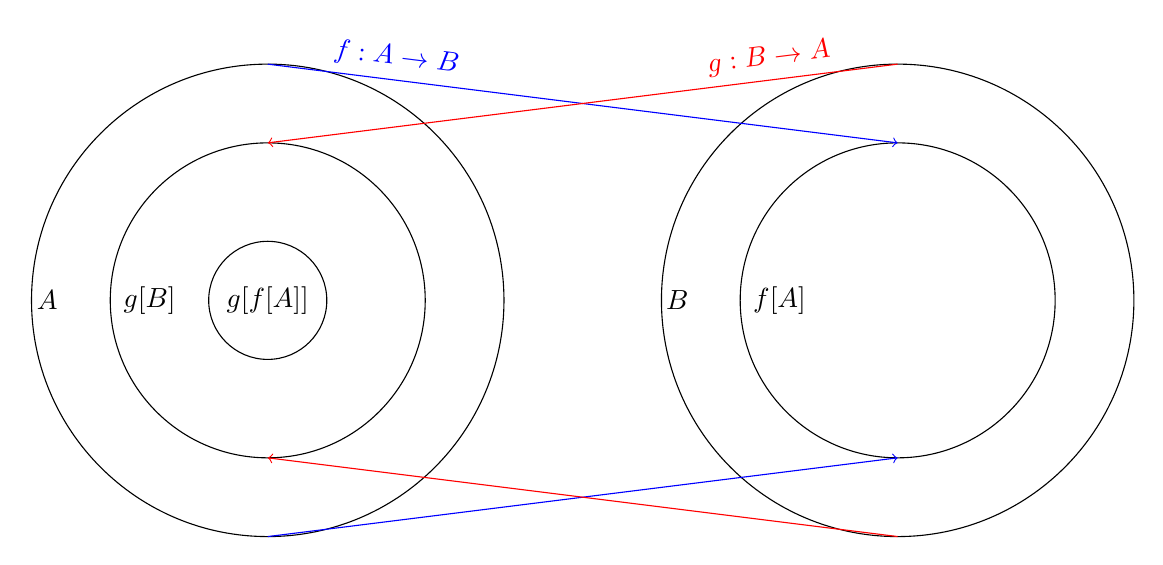
\begin{tikzpicture}
			\draw (-4, 0) circle (3); \draw (-6.8, 0) node {$A$};
			\draw (-4, 0) circle (2); \draw (-5.5, 0) node {$g[B]$};
			\draw (-4, 0) circle (0.75); \draw (-4, 0) node {$g[f[A]]$};
			
			\draw (4, 0) circle (3); \draw (1.2, 0) node {$B$};
			\draw (4, 0) circle (2); \draw (2.5, 0) node {$f[A]$};
			
			
			\draw[->, thin, blue] (-4, 3) -- (4, 2) node[pos=0.2, sloped, above, blue] {$f: A\to B$};
			\draw[->, thin, blue] (-4, -3) -- (4, -2);
			
			\draw[->, thin, red] (4, 3) -- (-4, 2)  node[pos=0.2, sloped, above, red] {$g:B\to A$};
			\draw[->, thin, red] (4, -3) -- (-4, -2);
			
		\end{tikzpicture}
	\end{center}
	\caption{Grafik des Sachverhalts im Satz \ref{SatzCantorSchroederBernstein}}
	\label{CantorSchroederBernsteinGrafik}
\end{figure}


\subsection{Ordinalzahlen}

Es wurden bereits die Zahlen $0,1,2,\dots,n,\dots,\omega,\omega+1,\omega+2,\dots,\omega+\omega$ diskutiert, mit welchen sich in diesem Kapitel genauer befasst werden soll.

Ein \textit{Graph} ist ein Paar $(A, R)$ so, dass $R\subseteq A\times A$ ein binäre Relation ist.

\begin{definition}[Partielle Ordnungen]
	Eine \textit{partielle Ordnung} ist ein Graph $(A,<)$ so, dass $<$ irreflexiv und transitiv ist. Eine alternative Definition ist $(A,\leq)$, wobei $\leq$ reflexiv, transitiv und antisymmetrisch ist.
\end{definition}

Eine \textit{lineare Ordnung} $(A,<)$ ist eine partielle Ordnung so, dass für alle $a,b\in A$ entweder $a<b$, $a=b$ oder $b<a$ gilt.

Ein Graph $(A,R)$ ist \textit{fundiert}, wenn jede nicht-leere Teilmenge $B\subseteq A$ ein Element $b\in B$ enthält so, dass $\{a\in B : (a,b) \in R\}= \emptyset$.
Also: Eine partielle Ordnung ist fundiert, wenn jede nicht-leere Teilmenge $B\subseteq A$ ein $<$-minimales Element enthält.

\begin{definition}[Wohlordnungen]
	Eine \textit{Wohlordnung} $(A,<)$ ist eine fundierte lineare Ordnung so, dass für jedes $a\in A$ die Klasse $\downarrow a\coloneqq \{b\in A : b < a\}$ eine Menge ist.
	Eine Relation $R\subseteq A\times A$, bei der für ein beliebiges $b$ die Klasse $\{a\in A : (a,b)\in R\}$ eine Menge ist wird auch als mengenähnlich bezeichnet.
\end{definition}

\begin{lemma}
	Sei $(A,<)$ eine fundierte, mengenähnliche, partielle Ordnung. Dann existiert in $A$ keine unendliche absteigende Folge $(a_n)_{n\in \omega}$ mit $a_{n+1}<a_n$ für alle $n$, wobei $\omega$ die Menge der natürlichen Zahlen bezeichnet.
\end{lemma}

Bemerkung: $(a_n)_{n\in \omega}$, $f:\omega \to A$ mit $a_n\coloneqq f(n)$

\begin{proof}
	Wenn eine solche Folge existiert, dann ist $\{a_n : n\in \omega\}=f[\omega]\subseteq A$ eine nicht-leere Klasse ohne $<$-minimales Element. Da $f[w]\subseteq \{a_0\}\cup \downarrow a$ und $A$ mengenähnlich ist, ist $f[w]$ eine Menge. Dies ist aber ein Widerspruch zur Fundiertheit.
\end{proof}

Um zu zeigen, dass jedes Element einer fundierten, mengenähnlichen partiellen Ordnung $(A,<)$ eine Eigenschaft $\psi$ erfüllt zeigt man, dass für für jedes $a$, dass wenn $\psi$ für alle $b<a$ gilt, dann auch für $a$.

\begin{satz}[Induktionsprinzip]
	Sei $(A,<)$ eine fundierte, mengenähnliche partielle Ordnung. Dann gilt
	\begin{itemize}
		\item[a)] Jede nicht-leere Klasse hat ein $<$-minimales Element.
		\item[b)] Sei $X\subseteq A$ so, dass für alle $a\in A$ gilt: Wenn $\downarrow a \subseteq X$, dann ist $a\in X$. Es folgt, dass $X=A$.
	\end{itemize}
\end{satz}
\begin{proof}
	a): Sei $B\subset A, a\in B$. Wegen der Mengenähnlichkeit ist $\downarrow a$ eine Menge und aus dem Aussonderungsaxiom folgt, dass auch $X\coloneqq B \cap (\downarrow a \cup \{a\})$ eine nicht-leere Teil\textit{menge} von $A$ ist. Es folgt auch, dass $X$ ein minimales Element $b$ besitzt. 
	
	Behauptung: $b$ ist auch das $<$-minimale Element von $B$. Andernfalls gibt es ein $c\in B$ mit $c < b \leq a$. Da $b\in X \subseteq B$ würde aber auch $c\in X$ folgen. Widerspruch!
	
	b): Annahme: $X$ sei wie gefordert, aber $X\neq A$. Also existiert ein $a\in A\setminus X$. Definiere $B\coloneqq \downarrow a \cup \{a\} \setminus \{X\}$. Dies ist eine nicht-leere Teilmenge und hat daher ein minimales Element $b$. Also ist $\downarrow b\subseteq A\setminus B\subseteq X$ und daher ist $b\in X$. Widerspruch!
\end{proof}

\begin{definition}[Ordinalzahlen]
	Eine \textit{Ordinalzahl} ist eine transitive Menge, welche durch $\in$ linear geordnet ist. 
	Beispiele sind $[n]$ für beliebige $n$, $\omega$, $\omega \cup \{\omega\}$. Die Klasse aller Ordinalzahlen ist $On$
\end{definition}

\begin{lemma}
	Ordinalzahlen sind wohlgeordnet durch $\in$.
\end{lemma}
\begin{proof}
	Sei $\beta\subseteq \alpha\in On$ und $\beta\neq \emptyset$. Da $\beta$ fundiert ist existiert ein $\gamma\in \beta$ mit $\gamma\cap \beta =\neq$. Also ist $\gamma$ kleinstes Element in $\beta$ bezüglich. $\in$
\end{proof}

\begin{definition}[Anfangsstück]
	Ein \textit{Anfangsstück} einer Ordnung $(A,<)$ ist eine Teilmenge $I\subseteq A$ so, dass $a\in I$ und wenn $b<a$, dann folgt $b\in I$. Ein Anfangsstück von $On$ ist also eine Teilmenge $$
\end{definition}

\end{document}













